% Appendix G — RQ3 extended results (quarterly trend + native-pool robustness)
% Companion to RQ3 ($\widehat{\rbt^A - \rbt^H}$ in \S\ref{sec:results}). For
% each PR-creation quarter in the analysis window we recompute the within-PR
% DiD under the same stable doubly-engaged cohort definition, separately for
% the (cross-family) Any-AI-vs-human cohort and the (within-family) Claude-
% vs-human cohort. 95\% CIs are analytical (rate-difference scale; two
% independent gaps summed in quadrature). The figure replicates Figure~2 on
% the symmetric (native-only) AI review pool, pooled across all four
% quarters.

\paragraph{Quarterly trend.} The cross-family within-PR DiD ($\widehat{\rbt^A - \rbt^H}$, AI bot reviewer vs.\ human reviewer on AI- vs.\ human-authored PRs) is negative in every quarter of the analysis window --- AI bots are systematically less approving of AI-authored code than humans are --- but its magnitude attenuates from \PLACEHOLDERRQ3QCFDID1{}~pp (95\% CI [\PLACEHOLDERRQ3QCFDIDLO1{}, \PLACEHOLDERRQ3QCFDIDHI1{}]) in 2025-Q2 to \PLACEHOLDERRQ3QCFDID4{}~pp ([\PLACEHOLDERRQ3QCFDIDLO4{}, \PLACEHOLDERRQ3QCFDIDHI4{}]) in 2026-Q1, even as the AI-authored cell grows from \PLACEHOLDERRQ3QCFNAI1{} to \PLACEHOLDERRQ3QCFNAI4{} PRs (Table~\ref{tab:rq3-quarterly}, top); the gap on human-authored PRs is approximately stationary, so the attenuation is driven by AI-authored-PR approval rates rising toward the human reviewer's, not by humans becoming harsher on AI-authored code. The within-family Claude-vs-human DiD is consistent with zero in each quarter for which it is identifiable (the 2025-Q2 cell has zero Claude-authored PRs in the cohort): point estimates are \PLACEHOLDERRQ3QWFDID2{}~pp, \PLACEHOLDERRQ3QWFDID3{}~pp and \PLACEHOLDERRQ3QWFDID4{}~pp for 2025-Q3, 2025-Q4 and 2026-Q1 respectively, with the 2025-Q4 estimate dominated by a Claude-authored cell of \PLACEHOLDERRQ3QWFNC3{} PRs (Table~\ref{tab:rq3-quarterly}, bottom); only 2026-Q1's CI ([\PLACEHOLDERRQ3QWFDIDLO4{}, \PLACEHOLDERRQ3QWFDIDHI4{}]) is tight enough to rule out anything beyond a small in-family preference, consistent with the pooled within-family result in \S\ref{sec:results}. Restricting the AI review pool to native \texttt{APPROVED}/\texttt{CHANGES\_REQUESTED} review states only --- symmetric with the human side --- shrinks the cross-family AI-authored cell to \PLACEHOLDERRQ3QCFNNAI1{}, \PLACEHOLDERRQ3QCFNNAI2{}, \PLACEHOLDERRQ3QCFNNAI3{} and \PLACEHOLDERRQ3QCFNNAI4{} PRs across 2025-Q2 $\to$ 2026-Q1 and yields per-quarter DiDs of \PLACEHOLDERRQ3QCFNDID1{}~pp [\PLACEHOLDERRQ3QCFNDIDLO1{}, \PLACEHOLDERRQ3QCFNDIDHI1{}], \PLACEHOLDERRQ3QCFNDID2{}~pp [\PLACEHOLDERRQ3QCFNDIDLO2{}, \PLACEHOLDERRQ3QCFNDIDHI2{}], \PLACEHOLDERRQ3QCFNDID3{}~pp [\PLACEHOLDERRQ3QCFNDIDLO3{}, \PLACEHOLDERRQ3QCFNDIDHI3{}] and \PLACEHOLDERRQ3QCFNDID4{}~pp [\PLACEHOLDERRQ3QCFNDIDLO4{}, \PLACEHOLDERRQ3QCFNDIDHI4{}] respectively --- non-monotone point estimates whose CIs all cross zero, confirming that the headline negative DiD is identified off the regex-parsed verdict pool (\Cref{app:ai-verdict-regex}), not off native review states; the within-family Claude pool under the same restriction collapses to \PLACEHOLDERRQ3QWFNNC1{}, \PLACEHOLDERRQ3QWFNNC2{}, \PLACEHOLDERRQ3QWFNNC3{} and \PLACEHOLDERRQ3QWFNNC4{} Claude-authored PRs respectively and is uninformative for all but 2026-Q1 (\PLACEHOLDERRQ3QWFNDID4{}~pp [\PLACEHOLDERRQ3QWFNDIDLO4{}, \PLACEHOLDERRQ3QWFNDIDHI4{}]).

\begin{figure}[h]
    \centering
    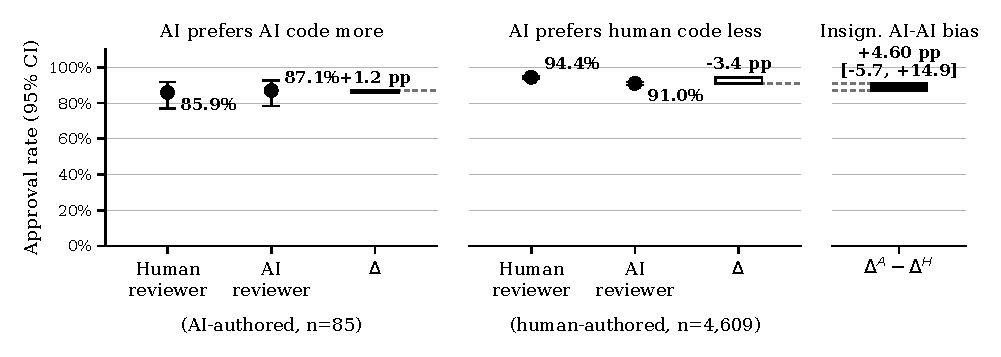
\includegraphics[width=\linewidth]{figures/figure2_withinpr_native.pdf}
    \caption{Within-PR DiD on the dual-review cohort, with the AI review pool restricted to native \texttt{APPROVED} / \texttt{CHANGES\_REQUESTED} review states only (symmetric with the human side). Pooled across the full Apr 2025--Mar 2026 window: \PLACEHOLDERRQ3QCFNPOOLNAI{} AI-authored and \PLACEHOLDERRQ3QCFNPOOLNH{} human-authored PRs. Same construction as Figure~\ref{fig:withinpr}. DiD $\widehat{\rbt^A - \rbt^H} = \PLACEHOLDERRQ3QCFNPOOLDID{}$~pp (95\% CI \PLACEHOLDERRQ3QCFNPOOLDIDCI{}) --- the headline negative result in \S\ref{sec:results} does not replicate in this small sample with only explicit review events included: the gap on AI-authored PRs is \PLACEHOLDERRQ3QCFNPOOLB1{}~pp [95\% CI \PLACEHOLDERRQ3QCFNPOOLB1CI{}] vs.\ a gap of \PLACEHOLDERRQ3QCFNPOOLB2{}~pp [95\% CI \PLACEHOLDERRQ3QCFNPOOLB2CI{}] on human-authored PRs, and the DiD's CI crosses zero.}
    \label{fig:withinpr-native}
\end{figure}

\begin{figure}[h]
    \centering
    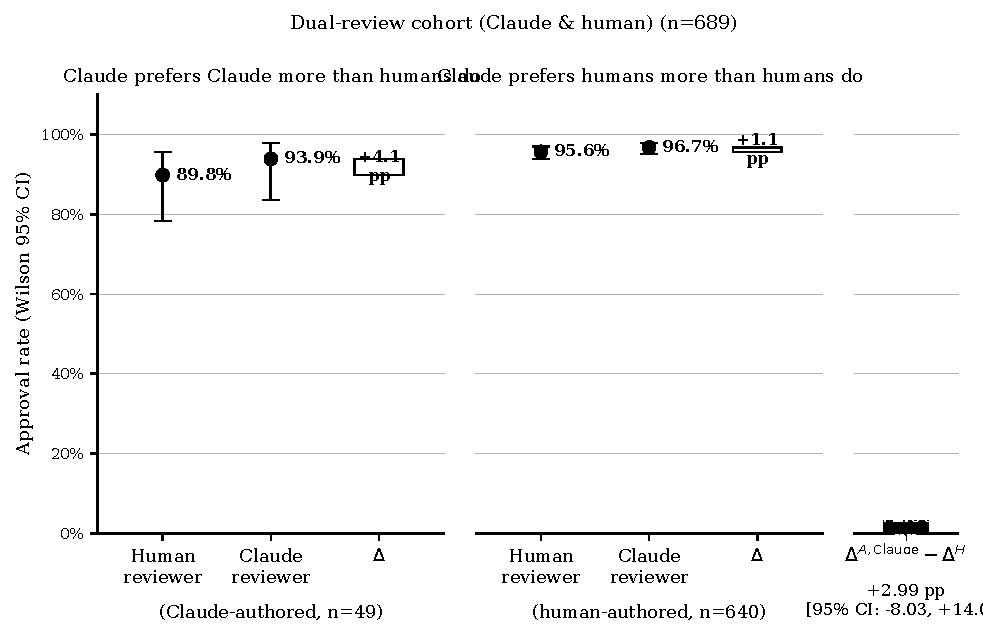
\includegraphics[width=\linewidth]{figures/figure2b_withinfamily_claude.pdf}
    \caption{Within-family check on the dual-review cohort (Claude \& human; \PLACEHOLDERRQ3BCNFOR{} PRs, \PLACEHOLDERRQ3BCAUTHOR{} Claude-authored). Same construction as Figure~\ref{fig:withinpr}. DiD $\widehat{\rbt^{A,\text{Claude}} - \rbt^H} = \PLACEHOLDERRQ3BDIDPP{}$~pp (\PLACEHOLDERRQ3BDIDPVAL{}) --- direction-consistent with a small in-family preference but indistinguishable from zero given the small Claude-authored cell.}
    \label{fig:withinfamily}
\end{figure}

\begin{table}[h]
\centering
\footnotesize
\setlength{\tabcolsep}{4pt}
\begin{tabular}{lrrrr}
\toprule
Quarter & 2025-Q2 & 2025-Q3 & 2025-Q4 & 2026-Q1 \\
\midrule
\multicolumn{5}{l}{\textbf{Cross-family: AI bot reviewer vs.\ human reviewer (RQ3 main)}} \\
PRs in cohort ($n$)               & \PLACEHOLDERRQ3QCFN1{}     & \PLACEHOLDERRQ3QCFN2{}     & \PLACEHOLDERRQ3QCFN3{}     & \PLACEHOLDERRQ3QCFN4{}     \\
\quad AI-authored cell ($n$)      & \PLACEHOLDERRQ3QCFNAI1{}   & \PLACEHOLDERRQ3QCFNAI2{}   & \PLACEHOLDERRQ3QCFNAI3{}   & \PLACEHOLDERRQ3QCFNAI4{}   \\
\quad H-authored cell ($n$)       & \PLACEHOLDERRQ3QCFNH1{}    & \PLACEHOLDERRQ3QCFNH2{}    & \PLACEHOLDERRQ3QCFNH3{}    & \PLACEHOLDERRQ3QCFNH4{}    \\
\multicolumn{5}{l}{\emph{On AI-authored PRs:}} \\
\quad AI rev.\ approval rate         & \PLACEHOLDERRQ3QCFAA1{}   & \PLACEHOLDERRQ3QCFAA2{}   & \PLACEHOLDERRQ3QCFAA3{}   & \PLACEHOLDERRQ3QCFAA4{}   \\
\quad Human rev.\ approval rate      & \PLACEHOLDERRQ3QCFHA1{}   & \PLACEHOLDERRQ3QCFHA2{}   & \PLACEHOLDERRQ3QCFHA3{}   & \PLACEHOLDERRQ3QCFHA4{}   \\
\quad gap (pp)                       & \PLACEHOLDERRQ3QCFB11{}   & \PLACEHOLDERRQ3QCFB12{}   & \PLACEHOLDERRQ3QCFB13{}   & \PLACEHOLDERRQ3QCFB14{}   \\
\qquad 95\% CI                       & \PLACEHOLDERRQ3QCFB1CI1{} & \PLACEHOLDERRQ3QCFB1CI2{} & \PLACEHOLDERRQ3QCFB1CI3{} & \PLACEHOLDERRQ3QCFB1CI4{} \\
\multicolumn{5}{l}{\emph{On human-authored PRs:}} \\
\quad AI rev.\ approval rate         & \PLACEHOLDERRQ3QCFAH1{}   & \PLACEHOLDERRQ3QCFAH2{}   & \PLACEHOLDERRQ3QCFAH3{}   & \PLACEHOLDERRQ3QCFAH4{}   \\
\quad Human rev.\ approval rate      & \PLACEHOLDERRQ3QCFHH1{}   & \PLACEHOLDERRQ3QCFHH2{}   & \PLACEHOLDERRQ3QCFHH3{}   & \PLACEHOLDERRQ3QCFHH4{}   \\
\quad gap (pp)                       & \PLACEHOLDERRQ3QCFB21{}   & \PLACEHOLDERRQ3QCFB22{}   & \PLACEHOLDERRQ3QCFB23{}   & \PLACEHOLDERRQ3QCFB24{}   \\
\qquad 95\% CI                       & \PLACEHOLDERRQ3QCFB2CI1{} & \PLACEHOLDERRQ3QCFB2CI2{} & \PLACEHOLDERRQ3QCFB2CI3{} & \PLACEHOLDERRQ3QCFB2CI4{} \\
DiD ($\widehat{\rbt^A - \rbt^H}$, pp) & \PLACEHOLDERRQ3QCFDID1{}  & \PLACEHOLDERRQ3QCFDID2{}  & \PLACEHOLDERRQ3QCFDID3{}  & \PLACEHOLDERRQ3QCFDID4{}  \\
\quad 95\% CI                       & \PLACEHOLDERRQ3QCFDIDCI1{}& \PLACEHOLDERRQ3QCFDIDCI2{}& \PLACEHOLDERRQ3QCFDIDCI3{}& \PLACEHOLDERRQ3QCFDIDCI4{}\\
\midrule
\multicolumn{5}{l}{\textbf{Within-family: Claude reviewer vs.\ human reviewer on Claude- vs.\ human-authored PRs}} \\
PRs in cohort ($n$)               & \PLACEHOLDERRQ3QWFN1{}    & \PLACEHOLDERRQ3QWFN2{}    & \PLACEHOLDERRQ3QWFN3{}    & \PLACEHOLDERRQ3QWFN4{}    \\
\quad Claude-authored cell ($n$)  & \PLACEHOLDERRQ3QWFNC1{}   & \PLACEHOLDERRQ3QWFNC2{}   & \PLACEHOLDERRQ3QWFNC3{}   & \PLACEHOLDERRQ3QWFNC4{}   \\
\quad H-authored cell ($n$)       & \PLACEHOLDERRQ3QWFNH1{}   & \PLACEHOLDERRQ3QWFNH2{}   & \PLACEHOLDERRQ3QWFNH3{}   & \PLACEHOLDERRQ3QWFNH4{}   \\
\multicolumn{5}{l}{\emph{On Claude-authored PRs:}} \\
\quad Claude rev.\ approval rate     & \PLACEHOLDERRQ3QWFAA1{}   & \PLACEHOLDERRQ3QWFAA2{}   & \PLACEHOLDERRQ3QWFAA3{}   & \PLACEHOLDERRQ3QWFAA4{}   \\
\quad Human rev.\ approval rate      & \PLACEHOLDERRQ3QWFHA1{}   & \PLACEHOLDERRQ3QWFHA2{}   & \PLACEHOLDERRQ3QWFHA3{}   & \PLACEHOLDERRQ3QWFHA4{}   \\
\quad gap (pp)                       & \PLACEHOLDERRQ3QWFB11{}   & \PLACEHOLDERRQ3QWFB12{}   & \PLACEHOLDERRQ3QWFB13{}   & \PLACEHOLDERRQ3QWFB14{}   \\
\qquad 95\% CI                       & \PLACEHOLDERRQ3QWFB1CI1{} & \PLACEHOLDERRQ3QWFB1CI2{} & \PLACEHOLDERRQ3QWFB1CI3{} & \PLACEHOLDERRQ3QWFB1CI4{} \\
\multicolumn{5}{l}{\emph{On human-authored PRs:}} \\
\quad Claude rev.\ approval rate     & \PLACEHOLDERRQ3QWFAH1{}   & \PLACEHOLDERRQ3QWFAH2{}   & \PLACEHOLDERRQ3QWFAH3{}   & \PLACEHOLDERRQ3QWFAH4{}   \\
\quad Human rev.\ approval rate      & \PLACEHOLDERRQ3QWFHH1{}   & \PLACEHOLDERRQ3QWFHH2{}   & \PLACEHOLDERRQ3QWFHH3{}   & \PLACEHOLDERRQ3QWFHH4{}   \\
\quad gap (pp)                       & \PLACEHOLDERRQ3QWFB21{}   & \PLACEHOLDERRQ3QWFB22{}   & \PLACEHOLDERRQ3QWFB23{}   & \PLACEHOLDERRQ3QWFB24{}   \\
\qquad 95\% CI                       & \PLACEHOLDERRQ3QWFB2CI1{} & \PLACEHOLDERRQ3QWFB2CI2{} & \PLACEHOLDERRQ3QWFB2CI3{} & \PLACEHOLDERRQ3QWFB2CI4{} \\
DiD ($\widehat{\rbt^{A,\text{Claude}} - \rbt^H}$, pp) & \PLACEHOLDERRQ3QWFDID1{}  & \PLACEHOLDERRQ3QWFDID2{}  & \PLACEHOLDERRQ3QWFDID3{}  & \PLACEHOLDERRQ3QWFDID4{}  \\
\quad 95\% CI                       & \PLACEHOLDERRQ3QWFDIDCI1{}& \PLACEHOLDERRQ3QWFDIDCI2{}& \PLACEHOLDERRQ3QWFDIDCI3{}& \PLACEHOLDERRQ3QWFDIDCI4{}\\
\bottomrule
\end{tabular}
\caption{Within-PR DiD (\S\ref{sec:results}) by PR-creation quarter. Top panel: cross-family DiD on the stable doubly-engaged Any-AI-and-human cohort. Bottom panel: within-family DiD on the Claude-and-human cohort, with author restricted to Claude or human (the 2025-Q2 Claude-author cell is empty in the cohort, so its DiD is undefined). The gap on each author-side row is the AI-reviewer approval rate minus the human-reviewer approval rate (in pp); the DiD is the gap on AI-/Claude-authored PRs minus the gap on human-authored PRs. 95\% CIs are analytical (two independent gaps summed in quadrature on the rate-difference scale).}
\label{tab:rq3-quarterly}
\end{table}
